\begin{multicols}{2}[\subsection{Der erste Tag}]

Diese ersten Tage mag ich gar nicht. Weder den in meinem Kindergarten, noch den
ersten Tag in meiner Schule, und jetzt auch noch der erste Tag an der Uni. Aber
immerhin soweit habe ich es geschafft: Ich bin an der Universität als Student
eingeschrieben. Eine Sache, an die meine Kindergärtnerin bestimmt nie dachte,
als sie mich damals betrachtet hatte. Ich bin zu früh. Noch ganze zwanzig
Minuten bis zum Beginn der Orientierungseinheit. Ich bin nervös, obwohl ich
nicht mal weiß wieso: Das Unbekannte? Das wird es wohl sein.

Unendliche Weiten. Wir schreiben das Jahr \thisYear \dots\ Einen Moment muss
ich bei diesem Gedanken lächeln, doch die Wirklichkeit und meine Unruhe holen
mich schnell wieder ein.  Ich setze mich einfach erst einmal hin.  Auf diese
blöden großen Treppenstufen. (Später erfahre ich, dass man die Stufen \glqq die
Badewanne\grqq\ nennt.) Ein Blick auf die Uhr: Noch 15 Minuten. Ich gucke mich
um, ob noch andere da sind, die man sofort als Erstsemestler erkennt. Einer
sitzt rund fünf Meter entfernt: unauffällig, guckt ununterbrochen in die Luft;
so schön sind die Lampen hier nun auch wieder nicht. Mir halb gegenüber sitzt
eine braunhaarige Studentin, liest ein Buch, guckt manchmal auf, um den Eingang
zum Hörsaal 1 zu betrachten, höchstwahrscheinlich, ob es schon losgeht. Neben
ihr in der Ecke sitzt einer, der auf seinem Handy rumtippt. Bei der hektischen
Bewegung spielt er etwas, vermute ich.  Bestimmt Snake. Dann sitzen da noch ein
paar Studenten, die sich lautstark über irgendeinen Film unterhalten. Von denen
trägt einer eine Mappe mit der Aufschrift \glqq Quasihomogene
Flächensingularitäten\grqq. Was das wohl ist?

Noch zehn Minuten. Dieses Warten ist furchtbar. Etwas Lektüre wäre jetzt gar
nicht schlecht, um mich ein bisschen abzulenken. So wie es die Studentin macht.
Aber darauf bin ich vorbereitet. Mein Lieblingsbuch habe ich dabei. Als ich das
Buch aus meinem Rucksack hole, fällt mir der neue Umschlag auf. Jemand muss
gestern Abend noch das Buch in Papier eingeschlagen und wieder zurück in meinen
Rucksack gelegt haben: Weiß. Kein Muster. Nur zwei Worte stehen in großen
Lettern darauf.

\begin{center}
\scshape{Keine Panik!}
\end{center}

Jetzt muss ich grinsen. Weggewischt die Unruhe. Meine Schwester? Meine Eltern?
Wer weiß\dots\ Ich lese vergnügt ein paar Minuten meine Lieblingspassagen in
\glqq Per Anhalter durch die Galaxis\grqq: \\ \glqq \glq Die Antwort auf die
Große Frage...\grq\ -- \glq Ja...\grq\ -- \glq... nach dem Leben, dem Universum
und allem...\grq, sagte Deep Thought. \glq Ja...!\grq\ -- \glq...lautet...\grq\
-- \glq Ja...!!\grq\ -- \glq 42\grq, sagte Deep Thought mit unsagbarer
Erhabenheit und Ruhe. \glq 42!  Und?\grq, kreischte Luunquoal los. \glq Ist das
alles, nach siebeneinhalb Millionen Jahren Denkarbeit?\grq\grqq\ \\ und: \\
\glqq \glq Ja!  Ich werde euch diesen Computer entwerfen. Und ich werde ihn
euch auch benennen.  Und er soll heißen... die ERDE.\grq\ Phouchg glotzte Deep
Thought an. \glq Ein saublöder Name\grq, sagte er.\grqq

Wir werden von einem Studenten aufgerufen in den Hörsaal zu kommen. Schnell
packe ich das Buch weg und betrete danach endlich den Hörsaal 1. Ein Student
drückt mir ein Heft in die Hand, darauf eine Nummer: 17 -- Schade. Nicht 42.
Ich setze mich lieber nicht ganz nach vorne. In die Mitte, das ist gut. Der
Sitz ist hart, aber nicht unbequem.  Mann, ist der Hörsaal riesig; hier werde
ich also demnächst des öfteren sitzen und einem Professor zuhören.

Jemand setzt sich neben mich, die Studentin von vorhin, dabei legt sie ihr Buch
demonstrativ vor sich hin: \glqq Das Leben, das Universum und der ganze
Rest\grqq, lese ich auf dem Cover.  Ich glaube langsam, dieser erste Tag wird
gar nicht so schlecht.

\begin{center}
\vfill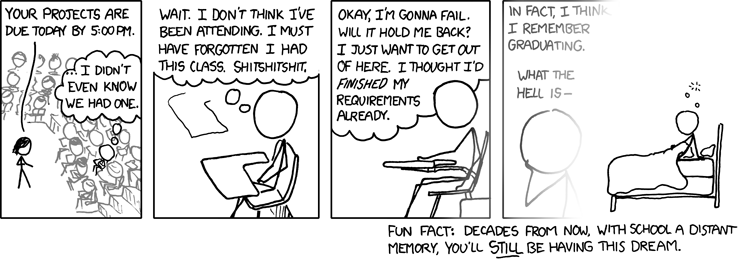
\includegraphics[scale=0.4]{comics/557}
\end{center}

\end{multicols}
